\documentclass[xcolor=dvipsnames]{beamer}

\usetheme{Berkeley}
%\usecolortheme{wolverine}

\newcommand{\bi}{\begin{itemize}}
\newcommand{\ei}{\end{itemize}}
\newcommand{\be}{\begin{enumerate}}
\newcommand{\ee}{\end{enumerate}}
\newcommand{\bc}{\begin{center}}
\newcommand{\ec}{\end{center}}
\newcommand{\I}{\item}
\newcommand{\f}{\frame}
\newcommand{\ft}{\frametitle}

\title{Hall D and IT}
\subtitle{at Internal Review of IT in the 12 GeV Era}
\author[M.\ Ito]{Mark M.\ Ito}
\date{May 20, 2011}
\institute[Hall D]{Hall D}

\begin{document}

\f{\titlepage}

\section{Introduction}

\f{
\ft{Hall D in a Nutshell}
\bi
\I search for exotic mesons in the 1.5 to 2.0 GeV region
\I 12 GeV electron beam
  \bi
  \I coherent bremsstrahlung photon beam
  \I coherent peak at 9 GeV
  \I photon tagger
  \ei
\I $4\pi$ detector: GlueX
  \bi
  \I charged tracking
  \I calorimetry
  \I particle ID (time of flight)
  \ei
\I amplitude analysis (a.k.a. partial wave analysis (PWA)) necessary
\ei
}

\f{
\ft{Topics: Aspects of Computing}
\bi
\I Requirements
\I Status of the Software
\I Planning, Tests, System Engineering
\ei
}

\section{Requirements}

\f{
\ft{Requirements}
\bi
\I attempt to capture all components of offline computation resources
\bi
\I Calibration
\I Reconstruction
\I Skimming
\I Analysis
\I Simulation
\ei
\I will not cover online computing
\bi
\I data acquisition software
\I software trigger
\ei
\I not all plans are fully formed
\I welcome comments on holes in planning
\ei
}

\f{
\ft{Raw Data}
\bi
\I strategy: take entire hadronic cross-section through level 1 trigger
\I start at photon intensity of $1\times10^7$/s in coherent peak
\I ramp to $1\times10^8$/s after ``two'' years
\I also ramp software trigger to give factor of 10 rejection
\I net effect: constant event rate to tape
\I 20~kHz when running
\I study: event size = 15~kB, instantaneous data rate = 300~MB/s
\I 35 weeks of running a year, 50\% running efficiency
\I average data rate: 200 billion events/year or 3.2~PB/year
\ei
}

\f{\ft{Calibration}\bi\I assume detectors can be calibrated using
  5\% of the raw data\bi\I gross simplification\I for estimating
  purposes\ei\I assume that calibrations will have to be done twice\ei}

\f{\ft{Reconstruction}
\bi
\I turning detector hits into particles
\I bulk of offline processing
\I 133~ms per event
\I assume output data 1/5 size of input data
\I assume that it needs to be done twice
\I do this at JLab
  \bi
  \I avoids shipping around raw data
  \ei
\ei
}

\f{\ft{Streaming}\bi\I dividing reconstructed events into separate
  ``streams'' for specific analyses\I based on event topology\I assume
  CPU load 1/10 that of reconstruction\I assume that number of events
  output 1/10 of that input\I assume five streams need to be
  produced\I must be done twice (like reconstruction)\ei}

\f{\ft{Analysis}
\bi
\I extraction of physics signals from reconstructed events
\I assume that CPU required is 1/10 of that needed to reconstruct (including repetitions factors)
\I multiple physics analysis, assume 10 of them
\I assume each analysis needs 20~TB of data on disk
\I statistical results, negligible storage requirements for output
\I PWA
  \bi
  \I highly CPU intensive
  \I suitable for off-site (modest data requirements)
  \I may require special resources (branch un-intensive: GPU farms)
  \I not included in this estimate
  \ei
\ei}

\f{\ft{Simulation}
\bi
\I create simulated data
\I assume reconstruction time same as that for raw data
\I generation time half of that to reconstruct
\I number events needed assumed to be twice raw data
  \bi
  \I want statistical error to be small compared to that of data,
  factor of 10 more\I more selective generation, factor of 5 less
  \ei
\I assume that it needs to be done twice
\I use of off-site resources is an option
  \bi
  \I collaborating institutions have farms
  \I grid paradigm established (OSG)
  \I other paradigms possible
  \ei
\I simulation studies outside this estimate
  \bi
  \I ideas often generated during analysis (creativity in science!)
  \I large demand for resources with desire for quick turn around
  \I grid-type environment well-suited for these cases 
  \ei
\ei
}

\f{\ft{Summary of Requirements}
\bc
\begin{tabular}{|l|r|r|r|}
\hline
Process & CPU (kCores$^a$) & Disk (TB) & Tape (PB/y)\\
\hline
Raw Data & -- & -- & 3.2 \\
Calibration & 0.09 & -- & 0.06 \\
Reconstruction & 1.8 & -- & 1.3$^b$ \\
Streaming & 0.9 & -- & 0.6 \\
Analysis & 0.9 & 200 & -- \\
Simulation & 5.4$^c$ & -- & 2.5$^b$ \\
\hline
Total & 9 & 200 & 8 \\
\hline
\end{tabular}
\ec
$^a$ single thread on a 2.8 GHz Nehalem machine \\
$^b$ roughly half may be able to be recycled \\
$^c$ significant amount may be done off-site \\
}

\section{Status of the Software}

\f{
\ft{Status of the Software}
\bi
\I Geometry
\I Simulation
\I Reconstruction
\I Partial Wave Analysis
\I Calibration Database
\I Data Format
\I Utilities
\ei
}

\f{
\ft{Geometry}
  \bi
  \I implemented in XML
  \I Hall D Detector Specification (HDDS)\bi
  \I XML elements and attributes closely follow GEANT defined shapes and their parameters\I mature\ei
  \I goal: keep the geometry in one place, use in
    \bi
    \I simulation (fully implemented)
    \I reconstruction (partially implemented)
    \I event display (to be implemented)
    \ei
  \ei
}

\f{
\ft{Simulation}
\bi
\I GEANT3-based: HDGEANT
  \bi
  \I geometry information auto-coded into FORTRAN code from HDDS information
  \I hits ({\it i. e.}, digitization) coded separately
  \I output in Hall Data Description Model format (HDDM, see slide below)
  \I mature
  \ei
\I experimental resolution added in separate stage: mcsmear
  \bi
  \I HDDM in, HDDM out
  \I in use
  \I development continues
  \ei
\I effort started to transition to GEANT4
\ei
}

\f{
\ft{Reconstruction}
\bi
\I JANA
  \bi
  \I multi-threaded: each thread a separate event stream
  \I algorithms for different detectors implemented as "factories"
  \ei
\I ROOT used for some general utilities
\I hooks for user code
  \bi
  \I user's class inherits from abstract base class
  \I must be registered with the framework
  \I multiple user classes possible
  \ei
\I plug-in mechanism
  \bi
  \I e. g., define user class at run time
  \ei
\I mature
\ei
}

\f{
\ft{Partial Wave Analysis (PWA)}
\bi
\I achieving physics goals of GlueX depends critically on PWA.
\I ``Collaborative Research: Open Access Amplitude Analysis on a Grid''
  \bi
  \I NSF-funded effort
  \I Carnegie Mellon, Indiana, Connecticut
  \ei
\I AmpTools 
  \bi
  \I PWA toolkit
  \I Indiana University
  \I GPU-based implementation
  \ei
\I Ruby-PWA
  \bi
  \I PWA toolkit
  \I Carnegie Mellon University
  \ei
\I plan to use off-site resources
\ei
}

\f{
\ft{Calibration Database}
\bi
\I relational database
\I based on CLAS experience (Hall B, JLab) with improvements
\I complete version history, with version choice at API level
\I facility for private versions, with history
\I tagging facility
\I code base exists
\I alpha testing next
\ei
}

\f{
\ft{Data Format}
\bi
\I raw data: EVIO
  \bi
  \I native CODA format
  \I mature
  \ei
\I simulation output: HDDM
  \bi
  \I Hall Data Description Model
  \I a compressed XML
  \I retains schema-like template at beginning of each file (uncompressed)
  \I C-based API, mature
  \I C++ API, in testing
  \ei
\I reconstruction output
  \bi
  \I options:
    \bi
    \I HDDM
    \I EVIO
    \I ROOT trees
    \ei
  \I need to finalize plans
  \ei
\ei
}

\f{
\ft{Utilities}
\bi
\I XML parsing: Xerces
\I source code management: subversion
\I source code documentation: doxygen
\I building scripts: GNU Make
\I database: MySQL
\I general documentation
  \bi
  \I GlueX Notes: DocDB
  \I webpages: mediawiki
  \ei
\ei
}

\section{Planning, Tests, System Engineering}

\f{
\ft{Planning, Tests, System Engineering}
\bi
\I Project Management
\I Simulation and Reconstruction Testing
\I Code Review--Repository Control
\I End-To-End Offline Test
\I Documentation
\I Communications
\I Off-Site Computing Facilitation
\ei
}

\f{\ft{Project Management}

\begin{columns}[c]
  \begin{column}{1.5in}
  \bi\I history\bi\I part of BIA\I captured in formal PM system\ei\I leverage this effort going forward\ei
  \end{column}
  \begin{column}{2.5in}
$$
  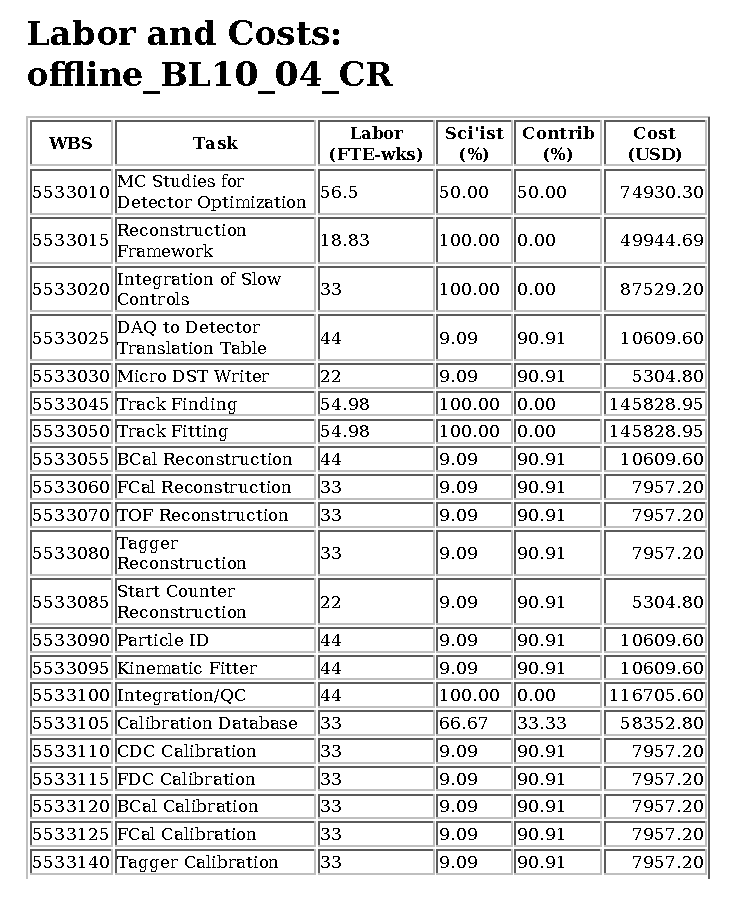
\includegraphics[height=3.0in]{pm.png}
$$
  \end{column}
\end{columns}
}

\f{
\ft{Simulation and Reconstruction Testing}
\bi
\I collaborators exercising code and generating feedback (now and forever)
\I analysis of simulated data underway
\I systematic reconstruction integrity
  \bi
  \I traditional approach: generate standard histograms
    \bi
    \I weekly simulation/reconstruction suite running in cron job
    \I only exotic meson channel simulated
    \ei
  \I to add: tests of individual software components
    \bi
    \I pinpoint problem areas
    \I major effort: coding the tests, generating appropriate test vectors
    \ei
  \ei
\ei
}

\f{
\ft{Code Review--Repository Control}
  \bi
  \I problem area
  \I worry that bad code gets checked in
  \I worry that restrictions inhibit productivity/creativity
  \ei
}

\f{
\ft {End-To-End Offline Test}
  \bi
  \I start in ET ring with raw data
  \I calibration, reconstruction, analysis
  \I need raw data format from DAQ group
  \I alternately, use HDDM surrogate for raw data
  \I resource-use-system development: need software just to use resources
  \I incremental development of test
  \I in conceptual stages
  \ei
}

\f{
\ft{Documentation}
\bi
\I major challenge
  \bi
  \I no one likes to write it
  \I critical to have it
  \ei
\I outline of formal system exists
\I on-going discussion
\ei
}

\f{\ft{Communications}
\bi
\I first-rate video conference capability
  \bi
  \I Hall D already a heavy user
  \I reflects investment of collaborating institutions
  \ei
\I remote viewing/inspection of experimental features
  \bi
  \I online/DAQ plots
  \I reading voltages
  \I {\it et cetera}
  \ei
\I actual control/change of parameters likely done by people physically in the counting room
\I locations at JLab:
  \bi
  \I counting house
  \I non-accelerator site locations
  \ei
\ei
}

\f{\ft{Off-Site Computing Facilitation}
\bi
\I need a way to ship data to and from JLab
\I will require resources
\I robust storage resource manager (SRM) is planned
\I grid utilities already installed at JLab
\ei
}

\section{Summary and Conclusions}

\f{\ft{Summary and Conclusions}
\bi
\I simulation and reconstruction is done routinely
\I positioned to exploit multi-core technology
\I computing model developed; will be iterated
\I many major components in place, others identified
\ei
\bc ...but... \ec
\bi
\I reconstruction still needs refinement
\I calibration not seriously addressed
\I adequate manpower a challenge
\ei
}

\end{document}

% end of latex file
